\documentclass[UTF8,11pt,a4paper]{ctexart}
\usepackage[a4paper,margin=2.3cm]{geometry}
\usepackage{amsmath,amssymb,amsthm}
\usepackage{booktabs}
\usepackage{graphicx}
\usepackage{float}
\usepackage[numbers]{natbib}
\usepackage{hyperref}
\usepackage{xcolor}
\usepackage{enumitem}
\usepackage{array}
\usepackage{longtable}
\usepackage{caption}
\usepackage{url}
\graphicspath{{figures/}{figures/peak_shaving_diagnostics/}{figures/peak_shaving_submission/}{figures/peak_shaving_smpt/}{./}}
\hypersetup{colorlinks=true,linkcolor=blue,citecolor=blue,urlcolor=blue}
\captionsetup{font=small}
\setlength{\emergencystretch}{3em}
\renewcommand{\abstractname}{摘要}
\renewcommand{\refname}{参考文献}

\newtheorem{proposition}{命题}
\newtheorem{remark}{说明}
\newtheorem{assumption}{假设}
\newtheorem{definition}{定义}
\newcommand{\qos}{q}
\newcommand{\T}{\mathcal{T}}
\newcommand{\M}{\mathcal{M}}
\newcommand{\D}{D}
\newcommand{\w}{\boldsymbol{w}}
\newcommand{\p}{\boldsymbol{p}}
\newcommand{\g}{\boldsymbol{g}}

\title{\textbf{固定容量推理服务分时定价的风格化仿真研究：\\
服务商竞争、QoS 保护与利润边界}}
\author{Anonymous Author}
\date{}

\begin{document}
\maketitle

\begin{abstract}
大语言模型（large language model, LLM）推理服务在短期内受到固定图形处理器（graphics processing unit, GPU）容量约束，而请求到达量在一天内存在明显波动。峰值过载会降低服务质量（quality of service, QoS），但离峰容量即使闲置也仍然产生持有成本。本文构建一个合成校准的风格化仿真模型，用于检验分时定价能否在不扩充容量的情况下，将时间弹性推理需求从拥塞时段转移出去并保护 QoS。模型包含两个异质推理服务商、一个应用程序编程接口（application programming interface, API）中间商、时间刚性用户与时间弹性用户、服务商直连 API 选项以及外部退出选项。服务商价格被限制在低维时间形状族内，竞争被表示为有限候选博弈，并用虚拟博弈和 regret 诊断评估。在拥塞设定下，统一定价使峰值利用率达到 $0.782$，最低 QoS 降至 $0.756$。动态粗网格和细网格快照分别将峰值利用率降至 $0.706$ 和 $0.666$，并将最低 QoS 提高至 $0.968$ 和 $0.990$。本文的主均衡证据来自完整 225 点网格上的双重 oracle 混合策略诊断；得到的 $5\times5$ 支撑集剖面最大 regret 为 $0.203$，期望峰值利用率为 $0.703$，最低 QoS 为 $0.970$。服务管理基线、结构消融、固定策略压力测试和受限局部重求解保持了正向 QoS 方向，但利润依赖求解对象：粗网格快照为 $+9.3\%$，细网格快照为 $-1.9\%$，低 regret 混合剖面约为 $-2.8\%$。因此，分时定价在本文中被解释为有边界的 QoS 保护机制，而不是生产预测或可靠的利润提升结果。
\end{abstract}

\noindent\textbf{关键词：} 推理服务仿真；分时定价；削峰；固定容量；API 中间商；QoS 保护；有限网格 regret

\section{引言}
\label{sec:intro}

大语言模型推理已经从离线批处理转向持续运行的在线服务。交互式聊天、代码生成、智能体工作流、周期性评测和定时批处理任务具有不同的日内到达模式。因此，GPU 推理集群会出现明显的峰谷负载波动，而这种波动难以通过短期容量扩张轻易消除 \cite{crankshaw2017clipper,gujarati2020clockwork,yu2022orca,kwon2023pagedattention,agrawal2024sarathiserve}。当利用率接近局部容量阈值时，首 token 时间（time to first token, TTFT）、排队延迟和完成率可能迅速恶化。QoS 下降会减少可完成并计费的请求量，同时降低用户满意度。

本文关注固定容量运行状态。GPU 采购与部署需要提前期，并伴随沉没成本；离峰闲置容量也会产生持有成本。在这种状态下，相比立即扩容，一种可操作替代方案是将价格作为需求塑形工具：提高峰时价格、降低离峰价格，并鼓励时间弹性需求向存在剩余容量的时段移动。这一动机与实时电价和需求响应相关 \cite{schweppe1988spot,borenstein2005long,albadi2008summary,faruqui2010household,siano2014demand}，但工程机制不同。推理服务质量受局部 GPU 利用率、延迟和完成率影响，而不是由发电约束或潮流方程决定。

推理服务市场也不同于简化定价模型中常见的单平台垄断。同一个开源模型族，例如 GLM，可以由多个服务商部署。当用户可感知的模型能力近似同质时，竞争主要由价格、可用容量和实际 QoS 驱动。服务商容量也存在异质性。较小服务商在中间商向其路由流量时可能更早进入拥塞区。这些观察促使本文构建一个市场层仿真模型：两个服务商提供近似同质但固定容量不同的推理服务，一个 API 中间商在两者之间路由流量，用户可以通过中间商购买、直接连接服务商 API，或退出市场。

本文有三点贡献。第一，提出一个固定容量推理服务的市场层仿真框架，在同一记账系统中表示服务商定价、中间商路由、用户退出和拥塞敏感 QoS。第二，将均衡证据明确限定为有限网格诊断：候选价格形状通过 QoS 固定点评估，虚拟博弈给出平均响应，单边偏离 regret 报告剩余可利用性。第三，识别服务质量效应和利润效应的分离。在拥塞校准下，分时定价在报告诊断中保持正向 QoS 方向，但利润效应符号随求解对象和扰动变化。因此，本文将分时定价定位为有边界的服务质量管理机制，而不是一般性的收入增强结果。

\section{相关研究综述}
\label{sec:related}

相关研究主要包括三类。第一，在线推理服务系统研究讨论了低延迟服务、批处理、内存管理、模型并行和 prefill/decode 分离 \cite{crankshaw2017clipper,gujarati2020clockwork,romero2021infaas,yu2022orca,li2023alpaserve,sheng2023flexgen,kwon2023pagedattention,agrawal2024sarathiserve,patel2024splitwise,zhong2024distserve,agrawal2024vidur}。这些研究解释了利用率升高时 QoS 为什么恶化，但通常没有把价格、用户退出和跨服务商竞争放入同一个市场层仿真模型中。

第二，拥塞定价和收益管理研究关注时变需求下的稀缺容量分配 \cite{vickrey1969congestion,arnott1990bottleneck,gallego1994dynamic,elmaghraby2003dynamic,bitran2003overview,talluri2004revenue,phillips2005pricing}。实时电价和需求响应进一步提供了削峰类比 \cite{schweppe1988spot,borenstein2005long,allcott2011rethinking,siano2014demand}。本文借鉴这一类文献的仿真报告顺序，即先定义用户、需求、容量和目标函数，再报告峰值负载、服务质量和敏感性结果。

第三，近期 AI 服务市场研究开始分析推理成本、菜单定价、token 容量合约和 GPU 服务的 Stackelberg 型定价 \cite{demirer2025emerging,erdil2025inference,bergemann2025menu,guo2026prillm,yan2026stackelberg,cunningham2026token,liu2026locational}。本文目标更窄：提供一个可复现的仿真框架，将 QoS 拥塞、服务商异质性、API 中间商、服务商直连选项和用户退出共同表示出来。用户选择遵循标准离散选择和平台市场工具 \cite{mcfadden1974conditional,anderson1992discrete,train2009discrete,rochet2003platform}。

\section{方法论}
\label{sec:model}

\paragraph{市场结构与决策顺序。}

一天被划分为 $T$ 个时段，$\T=\{1,\ldots,T\}$，每个时段长度为 $h$。仿真市场包含以下主体：
\begin{itemize}[leftmargin=2em]
  \item \textbf{两个异质推理服务商} $\M=\{A,B\}$，其固定容量满足 $G_A>G_B$。二者部署同一个开源模型，并被视为模型能力近似同质。服务商 $m$ 为中间商选择分时批发价 $w_{m,t}$，并为用户直连渠道选择分时零售价 $p^D_{m,t}$。
  \item \textbf{一个 API 中间商}，观察批发价格后选择分时零售价 $p_t$ 和路由权重 $r_{m,t}$，其中 $\sum_m r_{m,t}=1$。
  \item \textbf{两类用户}，按照 logit 随机效用模型，在中间商渠道、直连服务商 $A$、直连服务商 $B$ 和外部选项之间选择。
\end{itemize}
图~\ref{fig:market_schematic} 总结了决策顺序：服务商在 Nash 定价阶段同时发布价格，中间商计算其最优响应，随后用户选择与 QoS 通过拥塞固定点共同确定。

\begin{figure}[H]
\centering
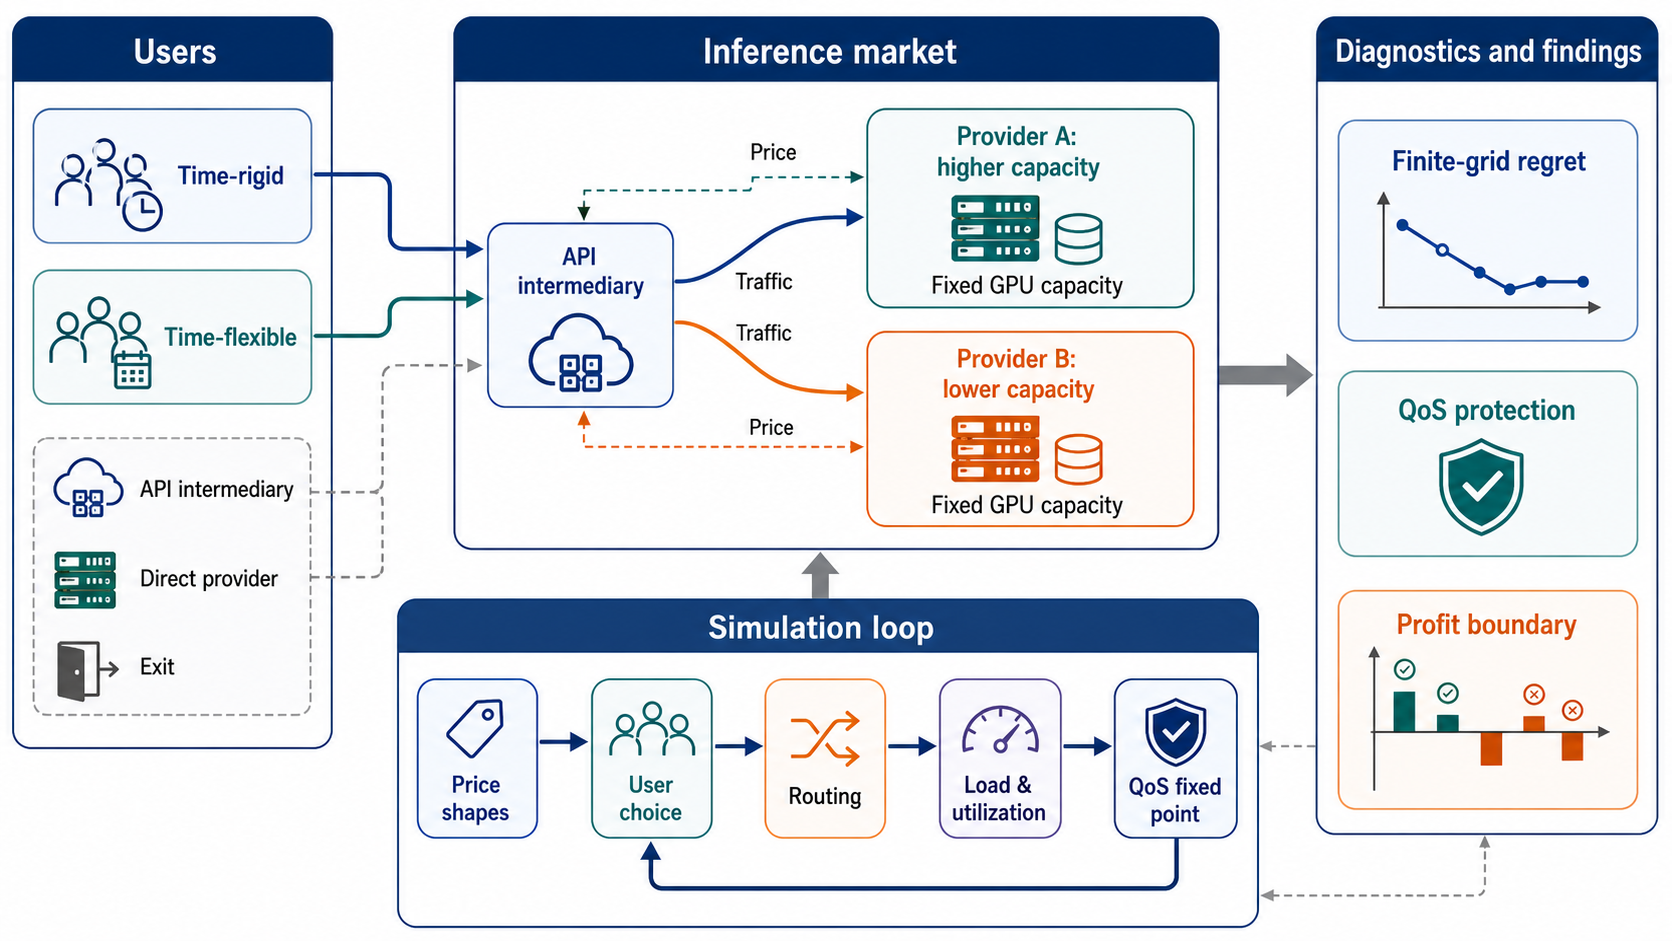
\includegraphics[width=\textwidth]{framework_imagegen_final_2026-07-10.png}
\caption{固定容量推理服务仿真框架。用户可以通过 API 中间商购买、直接连接服务商，或退出市场。中间商依据价格和 QoS 将流量路由到两个容量异质服务商。仿真循环依次评估价格形状、用户选择、路由、利用率和 QoS 固定点，诊断层报告有限网格 regret、QoS 保护和利润边界。}
\label{fig:market_schematic}
\end{figure}

\paragraph{用户选择与外部选项。}

存在两类用户 $\theta\in\{R,E\}$。类型 $R$ 用户为时间刚性用户，类型 $E$ 用户为时间弹性用户。对于渠道 $k$ 和时段 $t$，确定性效用定义为
\begin{equation}
  z^\theta_{k,t}=\log b_k+\log a_t
  -\alpha_\theta\!\left[\text{price}_{k,t}+c_s^\theta(1-\pi^\theta_t)-p_0\right]
  -\gamma(1-q_{k,t}).
  \label{eq:utility}
\end{equation}
其中，$b_k$ 表示渠道品牌价值或便利性，$a_t$ 表示时段偏好，$\pi^\theta_t$ 是类型 $\theta$ 的原生时段分布，$q_{k,t}$ 为渠道 QoS。迁移成本以价格等价单位表示，因此由同一个价格敏感度参数 $\alpha_\theta$ 缩放。选择集合由渠道--时段组合和外部选项构成。原生时段分布并不表示一个硬性的顺序到达过程，而是通过式~(\ref{eq:utility}) 表示偏离类型偏好时段的服务或 replay 成本。因此，本文中的“时间刚性”表示高迁移成本和峰时集中偏好，而不是完全无法跨时段移动；时间弹性用户价格敏感度更高、迁移成本更低，且原生时段分布更分散。

logit 分母包含一个不购买的外部选项，其确定性效用为 $u_0$。类型 $\theta$ 用户在时段 $t$ 选择渠道 $k$ 的份额及相应退出概率为
\begin{equation}
  s^\theta_{k,t}=\frac{\exp(z^\theta_{k,t})}{\exp(u_0)+\sum_{k',t'}\exp(z^\theta_{k',t'})},
  \qquad
  s^\theta_0=\frac{\exp(u_0)}{\exp(u_0)+\sum_{k',t'}\exp(z^\theta_{k',t'})}.
  \label{eq:share}
\end{equation}
内部份额之和小于一；剩余质量 $s^\theta_0$ 被解释为真实市场退出，而不会被重新分配到可购买选项。因此，价格上升可能减少内部需求，而不仅仅是在服务商或渠道之间重新分配需求。

\paragraph{需求、负载与 QoS。}

类型 $\theta$ 用户对渠道 $k$ 的需求由弹性成分和刚性/replay 成分组成。两个成分都由该渠道自身选择份额分配，这避免了一个时段内刚性总量随着可选渠道数量增加而缩放：
\begin{equation}
  \D^\theta_{k,t}=\bar F_\theta\,m^\theta(\p,q)\,s^\theta_{k,t}
  +\bar R^\theta_t\,\sigma[\beta(v_r-\text{price}_{k,t})]s^\theta_{k,t}.
  \label{eq:demand}
\end{equation}
其中 $\sigma(x)=(1+\exp[-x])^{-1}$。在实现中，弹性市场规模乘子为
\begin{equation}
  m^\theta(\p,q)
  =
  1+\eta\,[p_0-\bar p_\theta(\p,q)]_+,
  \qquad
  \bar p_\theta(\p,q)
  =
  \frac{\sum_{k,t}s^\theta_{k,t}(\p,q)\,\text{price}_{k,t}}
       {\sum_{k,t}s^\theta_{k,t}(\p,q)} ,
  \label{eq:market_size}
\end{equation}
主校准中 $\eta=1.2$。刚性/replay 响应在主校准中使用 $v_r=1.80$ 和 $\beta=5.0$。式~(\ref{eq:demand}) 应理解为一个紧凑的仿真装置，而不是用户到达过程的结构估计：logit 份额决定需求由哪个渠道和时段服务，原生时段项惩罚时间位移，replay 项则加入与时段负载相关的价格敏感残余需求。总需求是两类用户需求按人口权重 $(\pi_R,\pi_E)$ 加权求和。模型不是固定总需求模型。外部选项允许内部需求收缩，弹性市场规模项允许低价下需求扩张。因此，后文关于利润边界的讨论是一种机制分解和数值诊断，而不是建立在固定总需求上的定理。

服务商 $m$ 在时段 $t$ 的负载等于直连需求加上路由至该服务商的中间商需求：
\begin{equation}
  L_{m,t}=\D^D_{m,t}+r_{m,t}\D^I_t,
  \qquad
  u_{m,t}=L_{m,t}/G_m,
  \qquad
  q_{m,t}=\qos(u_{m,t}).
  \label{eq:load}
\end{equation}
主实验使用平滑 sigmoid 型 QoS 退化函数：
\begin{equation}
  \qos(u)=
  \frac{1}{1+\exp\{\operatorname{clip}[30(u-\bar u),-50,50]\}},
  \qquad \bar u=0.82 .
  \label{eq:qos_function}
\end{equation}
其中 $\bar u$ 是退化曲线中心：低于该值时服务质量接近一，利用率接近并超过该值后 QoS 快速下降。由于 $G_B<G_A$，在相同进入负载下，小容量服务商更早达到较低 QoS。阈值型、线性型和平方根型形状作为工件集中的稳健性检查保留。给定路由矩阵时，QoS 固定点通过阻尼迭代计算：
\begin{equation}
  \tilde q^{(n+1)}_{m,t}
  =\qos\!\left(\frac{L_{m,t}(q^{(n)})}{G_m}\right),
  \qquad
  q^{(n+1)}_{m,t}
  =(1-\lambda)q^{(n)}_{m,t}+\lambda \tilde q^{(n+1)}_{m,t},
  \label{eq:qos_fixed_point}
\end{equation}
报告实现中阻尼系数 $\lambda=0.35$，停止容差为 $10^{-9}$，迭代上限为 200 次。

\paragraph{包含固定容量持有成本的利润。}

服务商 $m$ 的利润等于批发收入加直连零售收入，减去固定容量持有成本和 QoS 退化成本：
\begin{equation}
  \Pi_m=h\!\sum_t\! w_{m,t}r_{m,t}\D^I_t q_{m,t}
  +h\!\sum_t\! p^D_{m,t}\D^D_{m,t}q_{m,t}
  -h\!\sum_t\! c_g G_m
  -h\!\sum_t\! c_q(1-q_{m,t})L_{m,t}.
  \label{eq:firm_profit}
\end{equation}
因子 $q_{m,t}$ 被解释为有效完成率或 SLA 达成因子。收入项乘以 $q_{m,t}$ 表示只有有效完成的需求被充分计费，这是一个偏保守设定。退化成本 $c_q(1-q_{m,t})L_{m,t}$ 表示服务降级导致的支持成本、声誉损失或合约惩罚，而不是一项独立观测到的会计支出。若生产 API 合约中失败请求仍可部分计费，则收入项会比本文设定更乐观。持有成本 $c_gG_m$ 作用于固定容量，而不是实际利用量。这使服务商有动机在低负载时段降价，以填充离峰容量。该设定区别于仅把容量作为固定上界、但忽略闲置资源成本的模型。

中间商渠道 QoS 和平均批发成本为
\begin{equation}
  q^I_t=\sum_m r_{m,t}q_{m,t},
  \qquad
  \bar w_t=\sum_m r_{m,t}w_{m,t}.
  \label{eq:intermediary_channel}
\end{equation}
其中间商利润为零售收入减批发成本和 QoS 退化成本：
\begin{equation}
  \Pi_I
  =h\sum_t p_t\D^I_t q^I_t
  -h\sum_t \bar w_t\D^I_t q^I_t
  -h\sum_t c_q(1-q^I_t)\D^I_t .
  \label{eq:intermediary_profit}
\end{equation}
系统利润为
\begin{equation}
  \Pi^{\mathrm{sys}}=\Pi_I+\sum_{m\in\M}\Pi_m .
  \label{eq:system_profit}
\end{equation}

\paragraph{求解方法与仿真诊断。}
\label{sec:solver}

\paragraph{低维价格形状族。}

如果每个服务商直接优化 $2T$ 个连续价格，即分时批发价和分时直连零售价，那么 Nash 博弈将是高维、非凸且难以数值复现的。因此，本文将服务商价格限制在低维时间形状族内：
\begin{equation}
  w_{m,t}=\bar w_m\big(1+\delta_m\widehat{\ell}_t\big),
  \qquad
  p^D_{m,t}=\bar p^D_m\big(1+\delta^D_m\widehat{\ell}_t\big).
  \label{eq:shape}
\end{equation}
向量 $\widehat{\ell}_t$ 是从刚性需求基线得到的零均值归一化负载形状，并被视为外生。每个服务商策略由四个标量 $(\bar w_m,\delta_m,\bar p^D_m,\delta^D_m)$ 表示。$\delta_m=0$ 对应统一定价，$\delta_m>0$ 表示峰时提价。该参数化牺牲了完整连续价格空间中的全局最优性，但提高了透明度、可重复性和诊断可控性。因此，除非另有说明，本文所有均衡语言均指该价格形状族内的均衡，不声称在不受限 $2T$ 维策略空间中达到全局最优。表~\ref{tab:solver_grids} 报告了求解诊断使用的有限网格。

\begin{table}[H]
\centering
\caption{求解诊断使用的有限候选网格}
\label{tab:solver_grids}
\small
\begin{tabular}{p{0.23\textwidth}p{0.37\textwidth}p{0.29\textwidth}}
\toprule
网格对象 & 候选取值 & 在论文中的作用 \\
\midrule
服务商粗网格 &
$\bar w\in\{0.30,0.85\}$，$\delta\in\{-0.4,-0.133,0.133,0.4\}$，$\bar p^D\in\{0.70,1.50\}$，$\delta^D\in\{-0.4,-0.133,0.133,0.4\}$ &
每个服务商 64 个策略形状，用于粗网格虚拟博弈诊断。 \\
服务商细网格 &
$\bar w\in\{0.27,0.575,0.88\}$，$\delta\in\{-0.4,-0.2,0,0.2,0.4\}$，$\bar p^D\in\{0.60,1.10,1.60\}$，$\delta^D\in\{-0.4,-0.2,0,0.2,0.4\}$ &
每个服务商 225 个策略形状，用于细网格快照和混合 oracle 扫描。 \\
中间商网格 &
$\bar p\in\{0.60,0.80,1.10,1.60\}$，$\delta_p\in\{-0.2,0,0.2\}$，$\beta_r\in\{1.5,4.0\}$ &
对每个服务商候选组合评估零售价和路由响应。 \\
\bottomrule
\end{tabular}
\end{table}

\paragraph{候选评估与有限博弈均衡证书。}

令 $s_m=(\bar w_m,\delta_m,\bar p^D_m,\delta^D_m)$ 表示服务商 $m$ 的价格形状策略，$\mathcal S_m$ 表示某一诊断中使用的有限候选网格。对于任意候选组合 $(s_A,s_B)$，式~(\ref{eq:shape}) 给出批发价和直连价。随后，中间商选择一个零售价格形状和路由敏感度，
\[
  y=(\bar p,\delta_p,\beta_r)\in\mathcal Y ,
  \qquad
  p_t=\bar p\big(1+\delta_p\widehat{\ell}_t\big),
\]
其中 $\mathcal Y$ 为中间商有限响应网格。给定 $y$ 后，路由作为批发价和服务商 QoS 的 logit 响应更新：
\begin{equation}
  r_{m,t}
  =
  \frac{\exp[-\beta_r w_{m,t}+\omega q_{m,t}]}
       {\sum_{j\in\M}\exp[-\beta_r w_{j,t}+\omega q_{j,t}]},
  \qquad \omega=3 .
  \label{eq:routing_logit}
\end{equation}
由于路由依赖 QoS，而 QoS 又依赖被路由负载，因此在中间商评估过程中，式~(\ref{eq:routing_logit}) 和式~(\ref{eq:qos_fixed_point}) 被作为联合阻尼固定点求解。中间商最优响应为
\begin{equation}
  y^\star(s_A,s_B)\in
  \arg\max_{y\in\mathcal Y}
  \Pi_I\big(s_A,s_B,y\big),
  \label{eq:intermediary_best_response}
\end{equation}
由此诱导的有限博弈中，服务商收益为
\begin{equation}
  U_m(s_A,s_B)=
  \Pi_m\big(s_A,s_B,y^\star(s_A,s_B)\big).
  \label{eq:finite_game_payoff}
\end{equation}

有限网格上的纯策略 Nash 均衡需要满足
\begin{equation}
  U_m(s_m^\star,s_{-m}^\star)
  \ge
  U_m(s_m,s_{-m}^\star)
  \quad
  \forall s_m\in\mathcal S_m,\quad m\in\M .
  \label{eq:pure_nash}
\end{equation}
本文不推导闭式 Nash 均衡，因为式~(\ref{eq:finite_game_payoff}) 中的收益由非线性 QoS 固定点、离散中间商响应和有限候选网格生成。相反，本文通过单边偏离 regret 报告可利用性。对于纯候选组合，
\begin{equation}
  \rho_m(s_A,s_B)
  =
  \max_{s'_m\in\mathcal S_m}U_m(s'_m,s_{-m})
  -U_m(s_m,s_{-m}),
  \qquad
  \rho(s_A,s_B)=\max_m\rho_m(s_A,s_B).
  \label{eq:pure_regret}
\end{equation}
对于有限网格上的混合剖面 $\mu=(\mu_A,\mu_B)$，期望收益和 regret 为
\begin{align}
  \bar U_m(\mu_A,\mu_B)
  &=
  \sum_{i,j}\mu_A(i)\mu_B(j)\,U_m(s_A^i,s_B^j), \label{eq:mixed_payoff}\\
  \rho_A(\mu)
  &=
  \max_i\sum_j\mu_B(j)U_A(s_A^i,s_B^j)
  -\bar U_A(\mu_A,\mu_B), \nonumber\\
  \rho_B(\mu)
  &=
  \max_j\sum_i\mu_A(i)U_B(s_A^i,s_B^j)
  -\bar U_B(\mu_A,\mu_B). \label{eq:mixed_regret}
\end{align}
零 regret 剖面将是有限候选博弈的混合 Nash 均衡。因此，报告值 $0.203$ 是有限网格可利用性证书，而不是不受限连续策略空间中的均衡证明。

\paragraph{虚拟博弈与有限网格 regret。}

服务商最优响应通过在四个价格形状参数上做网格搜索计算。网格搜索对非平滑 QoS 响应较稳健，计算预算可预测，并便于独立复现。中间商响应也通过网格搜索获得。每个候选评估都嵌入路由与 QoS 的联合固定点，并通过阻尼迭代求解。本文没有使用更深层的嵌套连续优化器，因为它在拥塞状态下会显著增加计算成本。

朴素最优响应迭代，即服务商交替对对方当前策略作最优响应，在拥塞状态下会产生循环行为。策略反复在两个配置之间切换，形成极限环。因此，本文使用虚拟博弈：每个服务商对对手运行平均策略作最优响应，而不是只响应最近一次策略。所得对象不是不受限纯策略 Nash 均衡，而是价格形状族内的时间平均虚拟博弈策略。只有当最大有利单边偏离，即 regret，足够低时，本文才将其视为可接受的均衡近似。参数漂移不作为主要收敛准则，因为它可能在粗网格上给出误导性的收敛印象。

对于细网格，本文增加双重 oracle 诊断。该过程从一个小候选集开始，在完整 225 点细网格上反复加入相对于当前混合剖面的最佳偏离，在受限支撑集上通过虚拟博弈求解经验混合剖面，最后扫描全网格计算 regret。

\begin{remark}[求解器校核与证据边界]
在非拥塞状态下，QoS 恒为一，固定点一次收敛，网格搜索是确定性的；系统利润的跨随机种子相对标准差为 $4.31\times10^{-4}$。拥塞状态需要单独的诊断边界。在粗网格上，虚拟博弈 regret 从 $133.6$ 单调下降到 $63.7$，最终降至 $4.98$，在 22 轮后达到 regret $<5$。在细网格纯策略快照中，regret 在第 10 轮附近达到约 $14$ 的局部最小值，随后上升，在 40 轮后漂移到约 $22$。新增的双重 oracle 混合诊断在完整 225 点细网格上得到一个 $5\times5$ 支撑集剖面，最终最大 regret 为 $0.203$。因此，QoS 改善作为有限网格混合/平均策略的低可利用性结果得到支持，但它不是不受限连续策略空间中的定理。
\end{remark}

\paragraph{校核、验证与可信度边界。}
\label{sec:vv}

在给定报告网格、参数设置和求解器种子的条件下，仿真是确定性的。校核（verification）关注实现是否遵循上文定义的记账、路由和固定点方程。验证（validation）的问题更窄：这些抽象是否足以可信地支持一个关于固定容量推理定价机制的研究。这些检查限定了本文主张，而不是认证一个生产推理服务或真实平台市场。

\paragraph{实现校核。}

实现将市场方程、QoS 固定点更新、中间商响应和服务商候选搜索分别放在独立模块中。主要校核依赖工件。在非拥塞设定下，QoS 为一且退化函数不激活，这校核了 QoS 模型的阈值以下分支。该状态下跨种子运行得到系统利润相对标准差 $4.31\times10^{-4}$。在拥塞设定下，报告工件保存静态基线、粗细候选响应、检查点轨迹、诊断图和混合策略 oracle 输出。

\begin{table}[H]
\centering
\caption{报告拥塞策略状态的固定点校核}
\label{tab:fixed_point_verification}
\small
\begin{tabular}{lccc}
\toprule
策略状态 & 是否收敛 & 迭代次数 & 最终残差 \\
\midrule
带 QoS 路由的静态定价 & 是 & 52 & $8.32\times10^{-10}$ \\
仅离峰折扣 & 是 & 32 & $8.23\times10^{-10}$ \\
仅峰时加价 & 是 & 34 & $9.71\times10^{-10}$ \\
动态粗网格 & 是 & 33 & $8.52\times10^{-10}$ \\
动态细网格快照 & 是 & 35 & $6.44\times10^{-10}$ \\
\bottomrule
\end{tabular}
\end{table}

表~\ref{tab:fixed_point_verification} 报告了主比较和服务管理基线诊断中使用的市场状态残差检查。另一个初始化与阻尼审计覆盖三个初始 QoS 水平和三个阻尼因子，作用于静态、动态粗网格和动态细网格状态。27 行中有 24 行收敛。动态粗网格和细网格在全部 18 个组合中均收敛。三行未收敛都出现在阻尼 $0.5$ 的静态拥塞基线中，其残差在 200 次迭代上限处仍约为 $0.312$。本文报告的静态基线本身使用默认阻尼 $\lambda=0.35$，并收敛到 $10^{-9}$ 以下。该审计没有穷尽网格搜索中的每个候选评估，但它校核了论文报告策略比较中使用的固定点状态，并识别了最拥塞静态情形下的数值边界。

\paragraph{验证与校准边界。}

公开 API 价格仅用于检查归一化价格尺度。它们不用于估计价格弹性、迁移成本或外部选项效用。受控 vLLM 过载测量仅用于锚定 QoS 退化代理的定性形状。测量使用一张 NVIDIA GeForce RTX 4090、两个 Qwen2.5 模型规模、短生成长度、每个并发水平五次重复，以及 0.5 秒 TTFT 服务水平协议（service-level agreement, SLA）阈值。它们支持阈值型 QoS 假设：服务在局部利用边界以下保持健康，在过载后恶化。它们不能替代真实到达轨迹、生产完成曲线、多 GPU 服务测量、长上下文工作负载或用户价格弹性估计。

敏感性证据分为三层。第一，固定策略压力测试扰动容量、价格敏感度、迁移成本和 QoS 阈值。第二，二维固定策略相图同时改变容量尺度和价格敏感度尺度。第三，对五个选定扰动运行受限局部候选重求解，其候选集由静态、动态粗网格、动态细网格、仅离峰折扣和仅峰时加价形状构成。最后一层是重求解仿真诊断，而不是全局均衡计算。

\paragraph{实验设计。}
\label{sec:setup}

仿真日包含 $T=8$ 个时段，每个时段 $h=3$ 小时。基线容量为 $G_A=1500$ 和 $G_B=600$。拥塞设定将容量收紧为 $G_A=300$ 和 $G_B=120$，以激活 QoS 退化。基线人口权重为 $(\pi_R,\pi_E)=(0.6,0.4)$；拥塞设定使用 $(0.4,0.6)$ 以提高峰时压力。所有经济参数均为合成校准。其数值用于支持机制分析，而不被解释为生产预测。表~\ref{tab:main_parameters} 总结了复现报告实验所需的主要参数。

\begin{table}[H]
\centering
\caption{报告实验使用的主要仿真参数}
\label{tab:main_parameters}
\small
\begin{tabular}{p{0.25\textwidth}p{0.23\textwidth}p{0.42\textwidth}}
\toprule
参数 & 取值 & 含义 \\
\midrule
$T,h$ & 8 个时段，3 小时 & 一个仿真日。 \\
$G_A,G_B$ & 1500, 600；拥塞 300, 120 & 服务商 A 和 B 的固定 GPU 服务容量。 \\
$(\pi_R,\pi_E)$ & 基线 $(0.6,0.4)$；拥塞 $(0.4,0.6)$ & 时间刚性和时间弹性用户的人口权重。 \\
$\alpha_R,\alpha_E$ & 2.0, 5.0 & logit 效用中的价格敏感度。 \\
$c_s^R,c_s^E$ & 0.60, 0.10 & 价格等价单位下的时段迁移成本。 \\
$p_0,v_r,\eta$ & 0.80, 1.80, 1.2 & 基准价格、刚性/replay 保留价值和弹性市场增长斜率。 \\
$\bar u,\gamma,c_q$ & 0.82, 1.0, 0.35 & QoS 阈值、QoS 效用权重和 QoS 退化成本。 \\
$c_g,u_0$ & 0.015, 0.0 & 固定容量持有成本和外部选项效用。 \\
\bottomrule
\end{tabular}
\end{table}

实验设计包含四层证据。第一层比较非拥塞和拥塞状态下统一定价与动态候选响应。第二层报告求解器诊断，包括纯策略 regret 和有限网格混合 oracle。第三层增加服务管理基线和结构消融。第四层使用固定策略压力测试、容量--弹性相图和受限局部重求解。主要输出指标包括峰值利用率、最低 QoS、服务量、系统利润、退出概率和 regret。该设计检验 QoS 机制，但不把每一个利润变化都视为稳健发现。

主要报告指标由固定点状态按如下方式计算：
\begin{align}
  u^{\mathrm{peak}}
  &=\max_{m,t}u_{m,t}, &
  q^{\min}
  &=\min_{m,t}q_{m,t}, \label{eq:reported_metrics}\\
  V^{\mathrm{served}}
  &=h\sum_{k,t}\D_{k,t}q_{k,t}, &
  \bar p^{\mathrm{paid}}
  &=
  \frac{\sum_{k,t}\text{price}_{k,t}\D_{k,t}q_{k,t}}
       {\sum_{k,t}\D_{k,t}q_{k,t}}, \nonumber\\
  \Delta \Pi^{\mathrm{sys}}
  &=
  \frac{\Pi^{\mathrm{sys}}_{\mathrm{policy}}-\Pi^{\mathrm{sys}}_{\mathrm{uniform}}}
       {\Pi^{\mathrm{sys}}_{\mathrm{uniform}}}\times100\%, &
  e_\theta&=s^\theta_0 . \nonumber
\end{align}
非拥塞诊断中的需求质心迁移定义为
\begin{equation}
  \Delta C_\theta
  =
  \frac{\sum_{k,t}t\,\D^\theta_{k,t}}{\sum_{k,t}\D^\theta_{k,t}}
  -
  \frac{\sum_{k,t}t\,\D^{\theta,\mathrm{uniform}}_{k,t}}
       {\sum_{k,t}\D^{\theta,\mathrm{uniform}}_{k,t}} .
  \label{eq:centroid_shift}
\end{equation}
因此，结果表中的数值是从仿真的固定点需求、利用率、QoS 和利润数组直接转换而来，而不是单独拟合得到的统计量。

公开 API 价格仅作为尺度参考。经核验的公开价格为：Z.AI GLM-4.7 输入每百万 token \$0.6、输出每百万 token \$2.2；DeepSeek-chat cache-miss 输入 \$0.27、输出 \$1.10；OpenAI GPT-4o 输入 \$2.50、输出 \$10.00 \cite{zaiPricing2026,deepseekPricing2026,openaiGpt4oPricing2026}。这些数值表明，仿真中使用的归一化价格与真实 API 价格处于相近数量级，但它们不用于估计需求弹性。完整参数值见补充材料。

本文复用两组受控 vLLM 单 GPU 过载测量来锚定 QoS 退化形状。后端为 vLLM 0.22.0，硬件为 NVIDIA GeForce RTX 4090，模型为 Qwen2.5-0.5B-Instruct 和 Qwen2.5-3B-Instruct。每个并发水平重复五次。QoS 观测定义为 TTFT 不超过 0.5 秒的 SLA 达成率。图~\ref{fig:vllm_qos_anchor} 显示，当归一化并发不超过一时，两条测量曲线都保持 SLA 达成率为一，并在健康并发点之后开始下降。对于 0.5B 模型，归一化并发为 $1.71$ 和 $2.29$ 时，SLA 达成率分别为 $0.635$ 和 $0.500$。对于 3B 模型，归一化并发 $1.71$ 时的达成率为 $0.667$。拟合阈值型函数 $q(u)=\exp[-\kappa(u-\bar u)^2_+]$ 后，0.5B 曲线得到 $(\bar u,\kappa,\mathrm{RMSE})=(1.000,0.517,0.068)$，3B 曲线得到 $(1.058,0.942,6.3\times10^{-10})$。这些测量为 QoS 代理提供验证式形状锚点，但不能替代真实请求轨迹、用户弹性估计或生产 SLA 校准。

\begin{figure}[H]
\centering
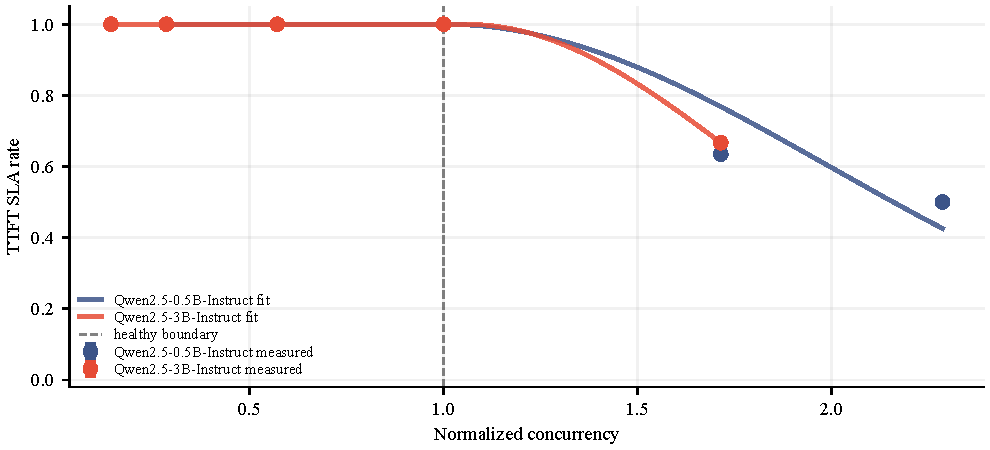
\includegraphics[width=0.88\textwidth]{vllm_qos_anchor.pdf}
\caption{作为 QoS 退化锚点的受控 vLLM 单 GPU 过载测量。横轴为按最大健康并发水平归一化后的并发量，纵轴为 0.5 秒 TTFT 阈值下的 SLA 达成率。点为五次重复测量的均值，线为拟合的阈值型 QoS 函数。}
\label{fig:vllm_qos_anchor}
\end{figure}

\section{实验结果}
\label{sec:results}

\paragraph{非拥塞状态。}

在基线容量下，市场未进入拥塞：统一定价下峰值利用率仅为 $0.213$，QoS 保持为一。表~\ref{tab:uncongested} 比较了统一定价与分时动态定价。

\begin{table}[H]
\centering
\caption{非拥塞状态：确定性网格搜索下统一定价与动态定价比较}
\label{tab:uncongested}
\begin{tabular}{lcc}
\toprule
指标 & 统一定价 & 动态定价 \\
\midrule
系统利润 & 1193.3 & 1139.4 \\
峰值利用率 & 0.213 & 0.261 \\
弹性需求质心迁移 & \multicolumn{2}{c}{$+0.177$} \\
刚性需求质心迁移 & \multicolumn{2}{c}{$+0.077$} \\
\bottomrule
\end{tabular}
\end{table}

需求迁移模式是稳定的。在动态定价下，时间弹性需求质心移动 $+0.177$ 个时段，而时间刚性需求质心移动 $+0.077$ 个时段。时间弹性需求的迁移幅度约为时间刚性需求的 $2.3$ 倍，符合预期机制。然而，由于非拥塞状态下 QoS 已经为一，质量改善空间很小。利润效应为中性至轻微负向：在弹性人口扫描中，收益变化分别为 $0\%$、$-0.32\%$、$-4.51\%$、$-3.76\%$ 和 $-3.00\%$。这表明分时定价的 QoS 保护作用只有在市场进入拥塞状态后才更有意义。

\paragraph{拥塞状态。}

容量收紧后，统一定价将市场推入拥塞。表~\ref{tab:congested} 将统一定价基线与主有限网格混合诊断放在一起。动态粗网格时间平均策略和动态细网格纯策略快照仍保留在表中，但仅作为求解器诊断，而不是同等意义的均衡对象。表~\ref{tab:evidence_boundary} 说明每个对象在论文主张结构中的使用方式。

\begin{table}[H]
\centering
\caption{拥塞状态：主比较与求解器诊断快照}
\label{tab:congested}
\small
\begin{tabular}{lcccc}
\toprule
指标 & 统一基线 & 主混合诊断 & 粗网格诊断 & 细网格诊断 \\
\midrule
峰值利用率 & 0.782 & 0.703 & 0.706 & 0.666 \\
最低 QoS & 0.756 & 0.970 & 0.968 & 0.990 \\
系统利润 & 1783 & 1733 & 1949 & 1749 \\
利润变化 & --- & $-2.8\%$ & $+9.3\%$ & $-1.9\%$ \\
最大 regret & --- & 0.203 & 4.98 & 22.30 \\
regret / 系统利润 & --- & $0.012\%$ & $0.26\%$ & $1.28\%$ \\
\bottomrule
\end{tabular}
\end{table}

\begin{table}[H]
\centering
\caption{拥塞状态的证据边界}
\label{tab:evidence_boundary}
\small
\begin{tabular}{p{0.25\textwidth}p{0.30\textwidth}p{0.35\textwidth}}
\toprule
对象 & 求解器状态 & 本文支持的主张 \\
\midrule
统一定价基线 & 虚拟博弈在 10 轮内达到准则 & 用作拥塞基线。 \\
动态粗网格 & 22 轮后 regret 为 $4.98$，但粗网格可能隐藏更细偏离 & 作为低分辨率诊断；不单独用于支持定量利润结论。 \\
动态细网格快照 & 40 轮后最大 regret 约为 $22.3$，高于 $<5$ 准则 & 仅用作分辨率压力测试和方向性比较；不解释为纯策略均衡。 \\
有限网格混合诊断 & 完整 225 点细网格扫描给出最大 regret $0.203$ & 支持有限网格混合/平均剖面的 QoS 结果；不外推到连续策略空间。 \\
\bottomrule
\end{tabular}
\end{table}

\begin{figure}[H]
\centering
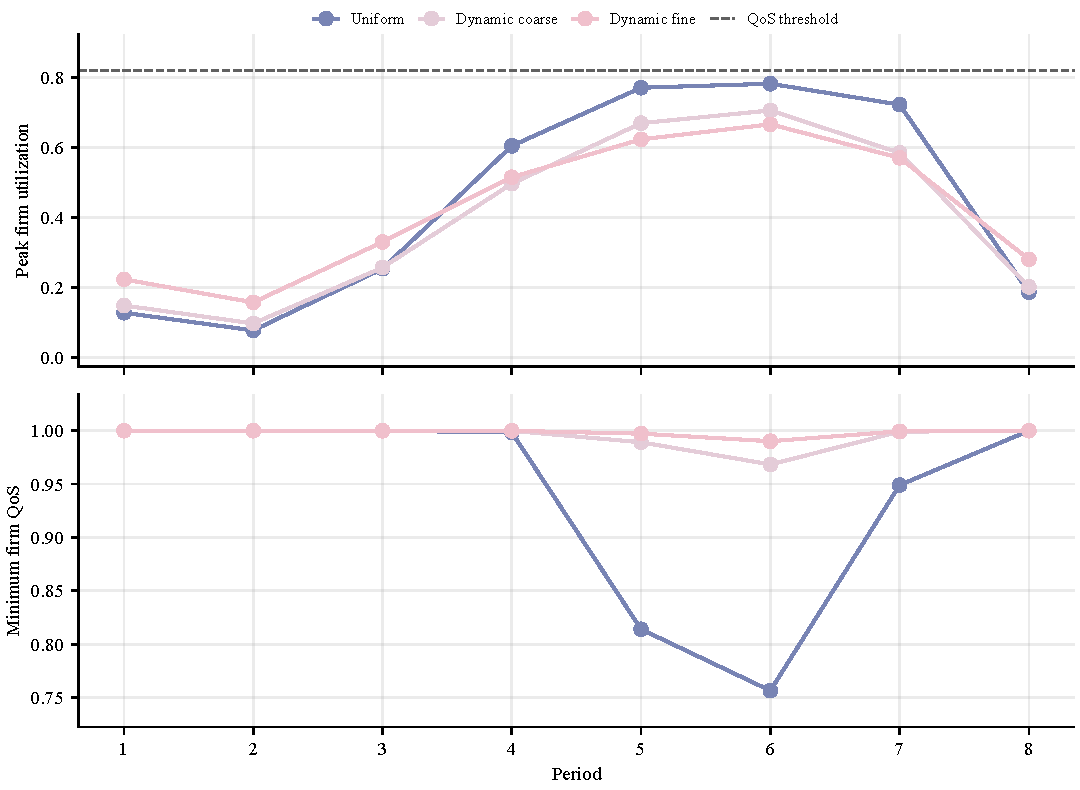
\includegraphics[width=0.86\textwidth]{qos_utilization_profiles.pdf}
\caption{拥塞状态下的时段利用率与 QoS 曲线。动态策略在粗网格和细网格快照中都降低峰值利用率并提高服务商最低 QoS。利用率面板中的虚线标示 QoS 退化曲线中心对应的利用率参数。}
\label{fig:qos_profiles}
\end{figure}

\begin{figure}[H]
\centering
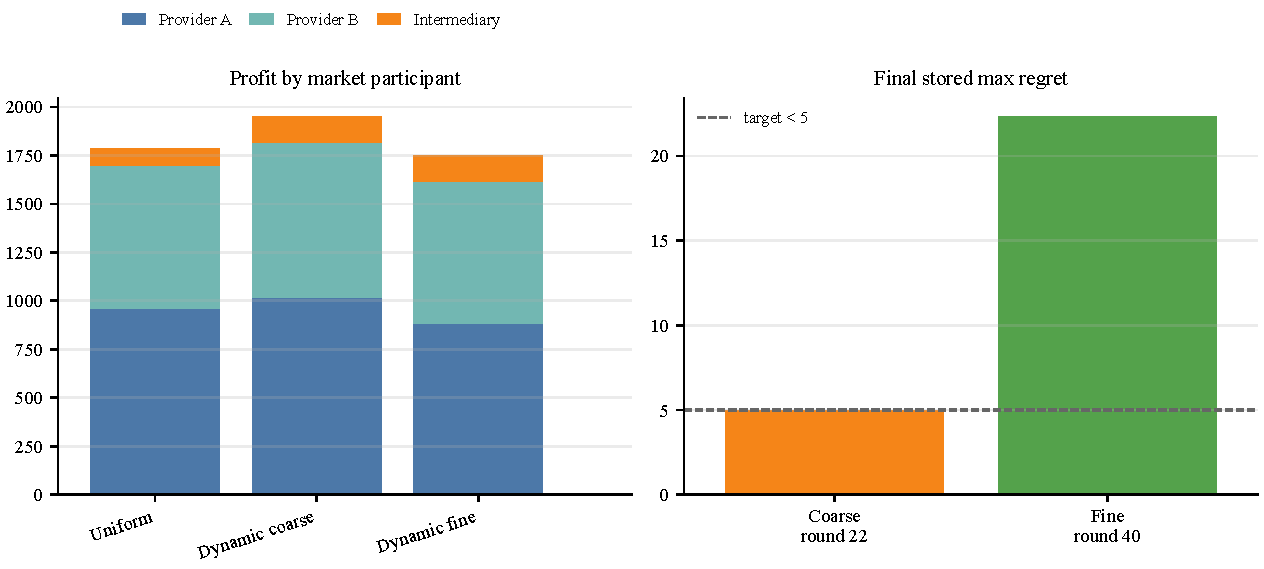
\includegraphics[width=0.88\textwidth]{profit_components_and_regret.pdf}
\caption{利润组成与纯策略 regret 边界。左图按市场参与者（服务商 A、服务商 B 和中间商）分解利润，右图报告已保存候选的最佳响应 regret。粗网格快照达到 regret $<5$，而细网格纯策略快照仍为 $22.3$，因此后者仅作为分辨率压力测试。}
\label{fig:profit_regret}
\end{figure}

\begin{figure}[H]
\centering
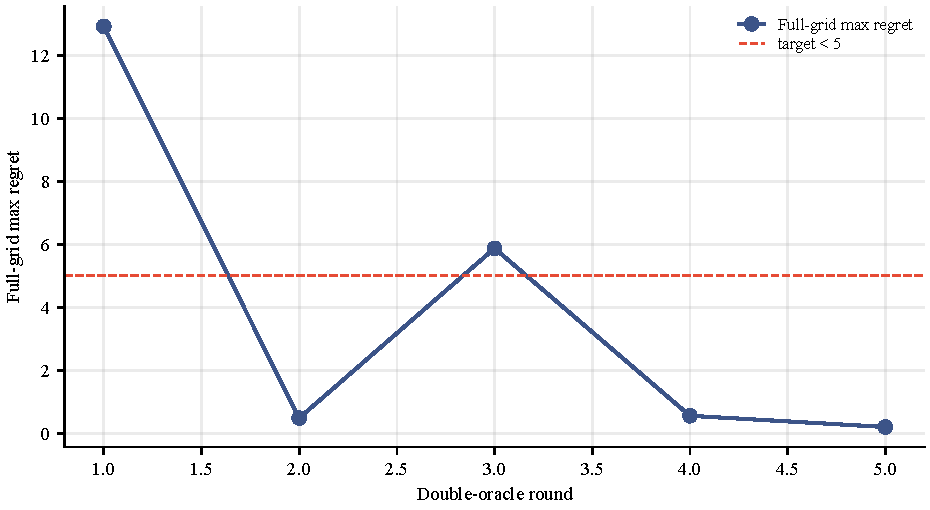
\includegraphics[width=0.76\textwidth]{mixed_oracle_regret.pdf}
\caption{双重 oracle 有限网格混合策略诊断。每一轮在完整 225 点细网格上加入相对于当前混合剖面的最佳偏离。第五轮得到 $5\times5$ 支撑集剖面，全网格最大 regret 降至 $0.203$。}
\label{fig:mixed_oracle}
\end{figure}

图~\ref{fig:qos_profiles}、图~\ref{fig:profit_regret} 和图~\ref{fig:mixed_oracle} 从时段、利润组成和 regret 角度展示同一组证据。中心比较是统一拥塞基线与低 regret 有限网格混合剖面。统一定价使最低 QoS 降至 $0.756$，峰值利用率升至 $0.782$；混合剖面的期望峰值利用率为 $0.703$，最低 QoS 为 $0.970$。粗网格和细网格快照显示相同 QoS 方向，但它们只作为求解分辨率诊断：粗网格分辨率较低，细网格快照仍具有较高 regret。因此，QoS 结论被表述为有限网格混合/平均剖面的结论，并在快照中检查方向一致性。

没有观察到稳健的正向利润效应。系统利润在粗网格快照中增加 $+9.3\%$，在细网格快照中下降 $-1.9\%$，在低 regret 混合剖面中约下降 $-2.8\%$。因此，本文不把利润提升作为正向发现。更稳妥的解释是，在当前求解预算和价格形状族内，分时定价具有 QoS 保护价值，但没有提供可靠正向利润增益的证据。

服务商异质性假设也并不稳定。一个自然猜想是，小容量服务商会更依赖动态定价，即 $\delta_B>\delta_A$。粗网格给出 $\delta_A=0.383$、$\delta_B=0.023$，而细网格给出 $\delta_A=0.059$、$\delta_B=0.278$。方向随网格分辨率反转。因此，本文不保留关于哪个服务商定价更动态的主张。需求迁移不对称性在非拥塞状态下同样清晰，但在拥塞求解对象中较弱：细网格情形下，弹性和刚性需求质心分别为 $4.23$ 和 $4.31$，差异很小。

\paragraph{服务管理基线诊断与结构检查。}

统一定价是有用基线，但单独使用可能偏弱。为检验 QoS 结果是否只是统一基线造成的假象，本文在拥塞设定周围增加四个服务管理诊断：仅离峰折扣、仅峰时加价、固定等路由下的动态粗网格定价，以及 admission-control 诊断。表~\ref{tab:smpt_baselines} 将这些基线与静态候选响应和两个主要动态快照放在一起报告。

\begin{table}[H]
\centering
\caption{拥塞设定下的服务管理基线诊断}
\label{tab:smpt_baselines}
\small
\begin{tabular}{lcccc}
\toprule
策略或诊断 & 峰值利用率 & 最低 QoS & 利润变化 & 服务量 \\
\midrule
带 QoS 路由的静态定价 & 0.782 & 0.756 & --- & 2610 \\
仅离峰折扣 & 0.766 & 0.833 & $+5.0\%$ & 2849 \\
仅峰时加价 & 0.738 & 0.921 & $+5.8\%$ & 2672 \\
动态粗网格 & 0.706 & 0.968 & $+9.3\%$ & 2865 \\
动态细网格快照 & 0.666 & 0.990 & $-1.9\%$ & 3043 \\
等路由动态粗网格 & 0.753 & 0.881 & $+5.9\%$ & 2817 \\
\bottomrule
\end{tabular}
\end{table}

单边价格形状基线改善了 QoS，但没有达到完整动态粗网格快照的水平。离峰折扣增加服务量，但留下更多峰时压力。峰时加价更直接降低峰值利用率，但恢复的服务量较少。等路由仍优于静态基线，但最低 QoS 仅为 $0.881$，而不是 $0.968$，表明价格时序和 QoS 感知路由都对报告结果有贡献。若使用统一价格 admission-control 诊断来匹配动态粗网格峰值利用率，则最紧张时段仅能接纳 $90.2\%$ 的需求，平均接纳率为 $97.4\%$。该诊断不是利润比较，但展示了通过限流而非定价达到类似峰值利用率目标时的服务质量代价。

\begin{table}[H]
\centering
\caption{动态粗网格策略的结构消融}
\label{tab:structural_ablations}
\small
\begin{tabular}{lccc}
\toprule
消融变体 & 最低 QoS 增益 & 峰值利用率下降 & 利润变化 \\
\midrule
基线模型 & $+0.212$ & $+0.076$ & $+9.3\%$ \\
无外部选项 & $+0.307$ & $+0.067$ & $+11.3\%$ \\
抑制服务商直连渠道 & $+0.000$ & $+0.209$ & $+0.0\%$ \\
同质容量 & $-0.054$ & $-0.154$ & $-3.6\%$ \\
无时间弹性用户 & $+0.155$ & $+0.046$ & $+6.1\%$ \\
固定等路由 & $+0.125$ & $+0.029$ & $+5.9\%$ \\
\bottomrule
\end{tabular}
\end{table}

表~\ref{tab:structural_ablations} 收窄了机制主张。动态粗网格策略在四个消融行中保持了实质性的正 QoS 增益。两个边界情形尤其有信息量。抑制服务商直连渠道使两种策略几乎都不拥塞，因此动态优势几乎消失。将服务商容量同质化则反转了动态优势，QoS 增益为 $-0.054$，利润变化为 $-3.6\%$。因此，当市场存在异质容量、服务商直连替代选项，且拥塞严重到足以使价格发挥作用时，结果最强。

\paragraph{局部参数压力测试。}

为检验 QoS 方向是否依赖单一合成校准，本文围绕拥塞基线评估四组局部扰动：容量尺度、价格敏感度、迁移成本和 QoS 阈值。在每个扰动点上，报告的统一、动态粗网格和动态细网格策略快照在不重新求解博弈的情况下被评估。因此，该练习是固定策略压力测试，而不是跨参数均衡陈述。

\begin{figure}[H]
\centering
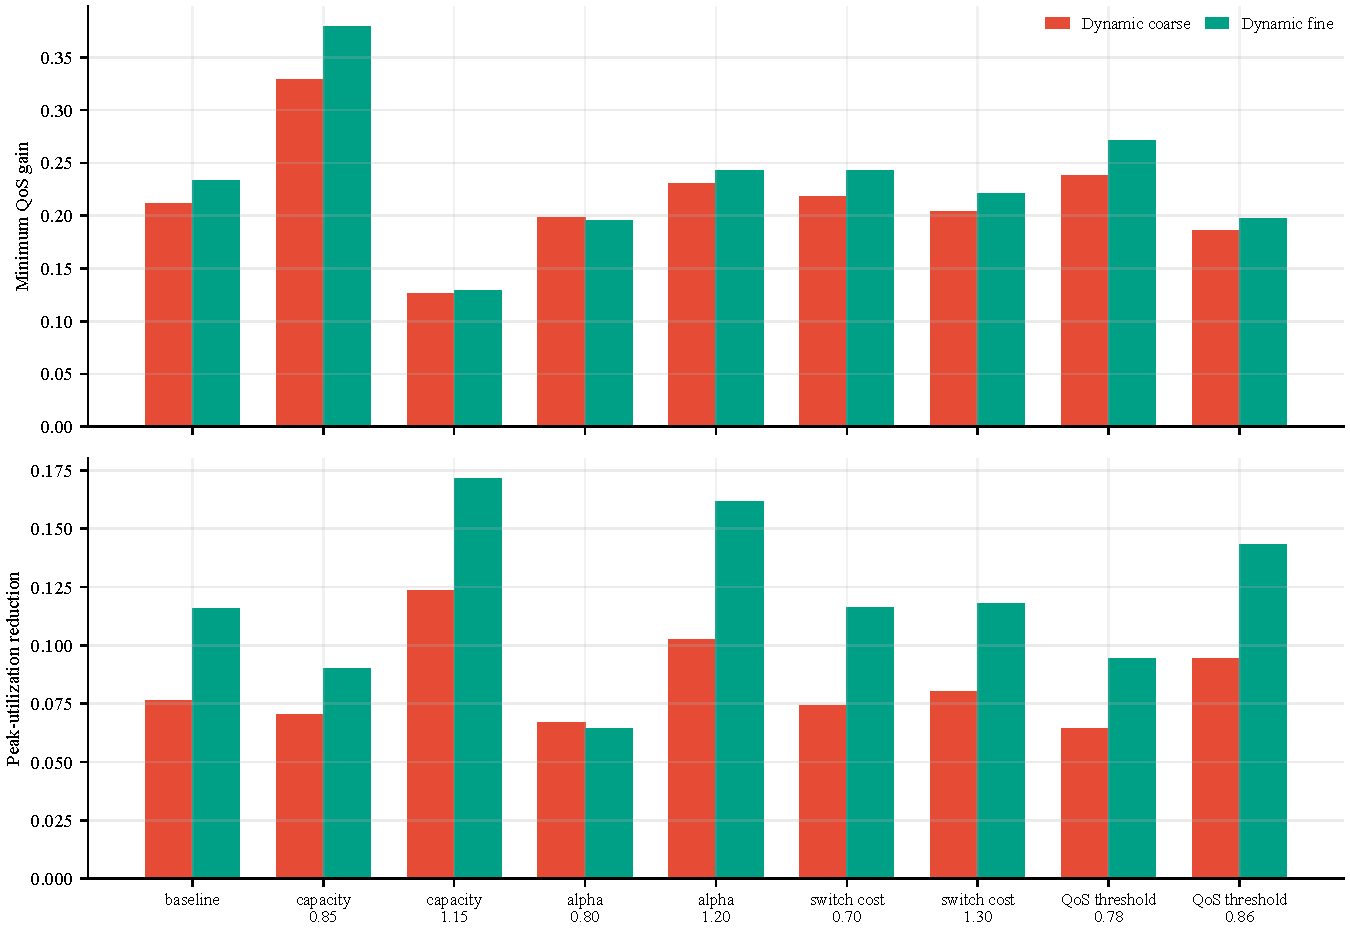
\includegraphics[width=0.92\textwidth]{parameter_sweep_qos.pdf}
\caption{参数压力测试。在九个扰动场景中，相对于统一定价，动态粗网格和动态细网格快照均保持正的最低 QoS 增益，并降低峰值利用率。}
\label{fig:parameter_sweep}
\end{figure}

图~\ref{fig:parameter_sweep} 显示，两个动态快照在九个扰动场景中都保持正 QoS 增益并降低峰值利用率。粗网格快照的最小最低 QoS 增益为 $0.126$，细网格快照为 $0.129$。利润仍不适合形成强正向结论：粗网格快照在九个场景中均为正利润，而细网格快照只有一个场景为正。该扫描支持 QoS 方向的局部固定策略稳健性，同时再次说明利润提升并不稳健。

\begin{figure}[H]
\centering
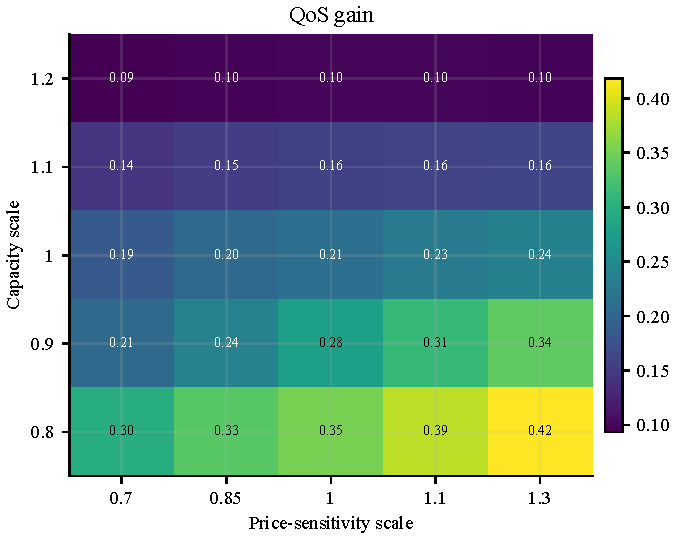
\includegraphics[width=0.48\textwidth]{smpt_phase_qos_gain.pdf}
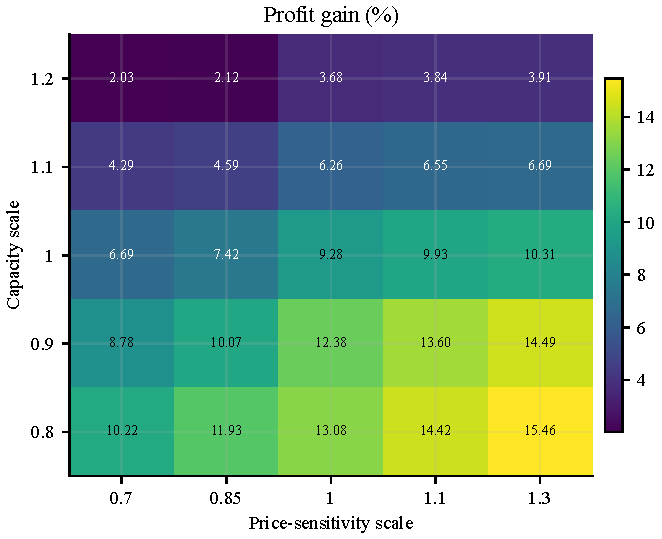
\includegraphics[width=0.48\textwidth]{smpt_phase_profit_gain.pdf}
\caption{容量尺度和价格敏感度尺度上的固定策略相图。动态粗网格策略在全部 25 个网格点上保持正 QoS 增益和峰值利用率下降。该固定策略网格上的利润为正，但表~\ref{tab:resolved_sensitivity} 中的受限重求解敏感性仍然混合。}
\label{fig:smpt_phase}
\end{figure}

图~\ref{fig:smpt_phase} 中的固定策略相图给出了更宽的局部视角。在全部 25 个容量--弹性网格点上，QoS 增益和峰值利用率下降均为正，最低 QoS 增益为 $0.094$。在这个固定粗网格策略相图上，利润为正，范围为 $+2.0\%$ 到 $+15.5\%$。这并不推翻利润边界结果，因为粗策略在这里被固定不变。

\begin{table}[H]
\centering
\caption{选定扰动下的受限局部重求解}
\label{tab:resolved_sensitivity}
\small
\begin{tabular}{lccc}
\toprule
场景 & 最低 QoS 增益 & 峰值利用率下降 & 利润变化 \\
\midrule
容量尺度 $0.90$ & $+0.280$ & $+0.060$ & $+12.5\%$ \\
价格敏感度尺度 $1.15$ & $+0.241$ & $+0.150$ & $-1.4\%$ \\
弹性用户占比 $0.70$ & $+0.242$ & $+0.136$ & $-1.9\%$ \\
QoS 阈值 $0.78$ & $+0.241$ & $+0.066$ & $+11.0\%$ \\
外部选项效用 $0.50$ & $+0.156$ & $+0.069$ & $+0.7\%$ \\
\bottomrule
\end{tabular}
\end{table}

在这一更强检查中，局部候选集包含静态、动态粗网格、动态细网格、仅离峰和仅峰时形状，每个场景运行四轮局部最优响应。表~\ref{tab:resolved_sensitivity} 在全部五行中都保持正 QoS 增益，增益范围为 $0.156$ 到 $0.280$。利润仍然混合。在当前设计下，这是对论文中心分离结论最具约束力的稳健性检查：QoS 方向在额外诊断中保持一致，而利润效应仍依赖参数和求解对象。

\section{总结展望}
\label{sec:discussion}
\label{sec:conclusion}

本文的中心发现很明确：在拥塞状态下，分时定价对 QoS 的保护比对利润的提升更稳定。最低 QoS 从 $0.756$ 提高到约 $0.97$ 或更高，而利润效应在粗网格快照、细网格快照和低 regret 混合剖面之间符号变化。因此，本文不把利润作为正向结果处理，而是将其作为诊断，用于解释为什么 QoS 改善并不必然转化为服务商利润。

\begin{figure}[H]
\centering
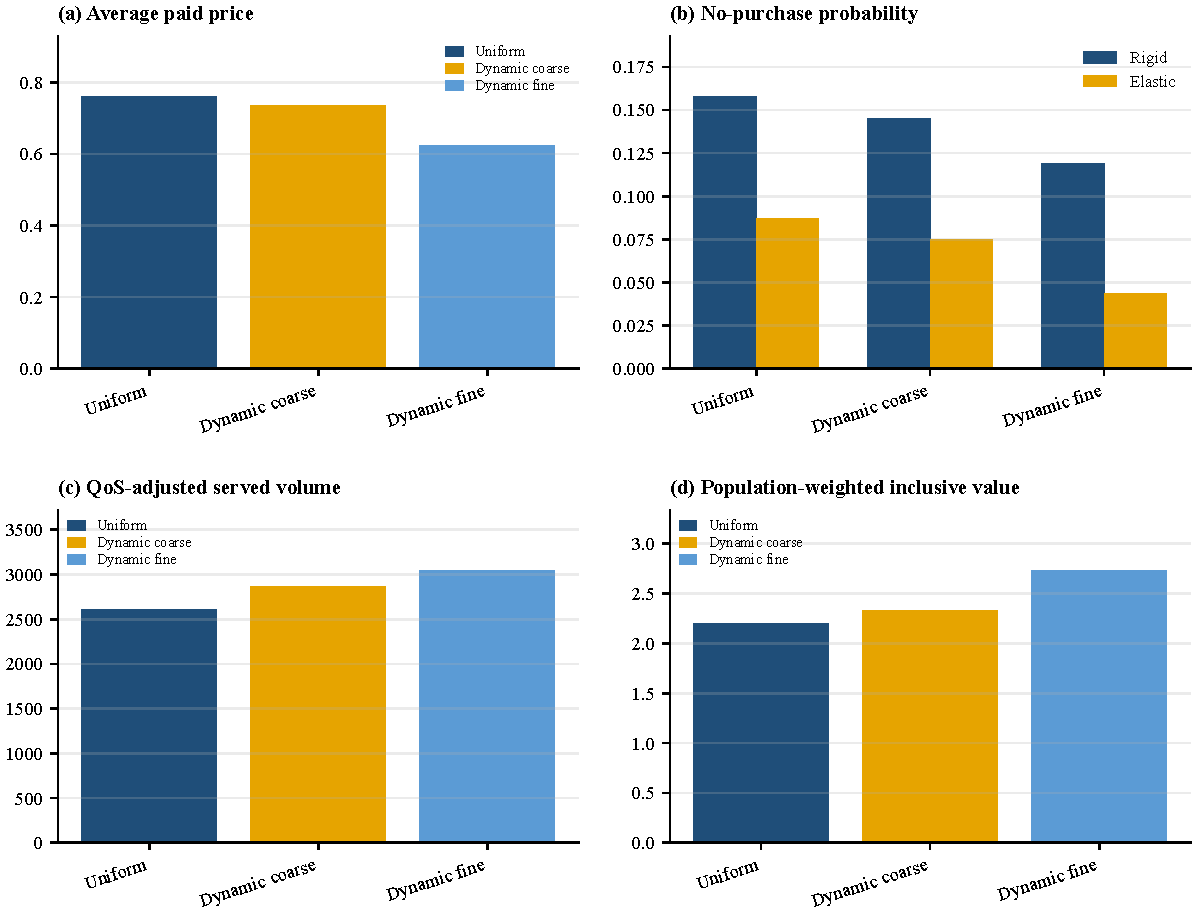
\includegraphics[width=0.9\textwidth]{mechanism_diagnostics.pdf}
\caption{拥塞状态下的机制诊断。面板 (a)--(d) 分别报告平均支付价格、无购买概率、QoS 调整后的服务量和人口加权 inclusive value。动态定价改善服务量和无购买结果，同时降低平均支付价格；这一模式与剩余重分配解释一致，而不是稳定的服务商利润增益。}
\label{fig:mechanism}
\end{figure}

\paragraph{剩余重分配而不是新增供给。}

固定容量是本仿真的核心约束。分时定价无法增加物理 GPU 供给，只能改变需求在时段和渠道之间的分布。图~\ref{fig:mechanism} 中的诊断与这一机制一致。在统一拥塞基线下，QoS 调整后的服务量为 $2610$。在动态粗网格和细网格快照下，该值分别增加到 $2865$ 和 $3043$。同时，时间刚性用户的退出概率从 $0.158$ 降至 $0.145/0.119$，时间弹性用户的退出概率从 $0.087$ 降至 $0.075/0.044$。这些数值表明，动态定价恢复了部分由拥塞造成的服务损失。混合策略诊断进一步表明，这一 QoS 方向不依赖单个高 regret 细网格点。

然而，恢复的服务量没有转化为稳健利润。主要原因是价格和数量方向相反：平均支付价格从 $0.761$ 降至 $0.735/0.625$。对于服务商，正向力量包括更高的峰时边际、离峰闲置容量利用改善，以及 QoS 恢复带来的有效计费量增加。负向力量也同时存在。峰时提价可能使价格敏感需求转向竞争者、直连选项或外部选项。离峰折扣降低单次请求边际。被峰时挤出的弹性用户也可能成为净流失需求。因此，峰时价格收益可能被需求损失抵消，新增离峰量也可能被更低边际抵消。

这一模式不应被理解为固定总需求下的定理。模型包含外部选项和价格响应的市场规模项，因此内部需求会随价格和 QoS 变化。更准确的解释是剩余重分配。分时定价主要在时段和渠道之间重新分配需求，而不是可靠地创造可被服务商完全攫取的新剩余。

\paragraph{为什么恢复的 QoS 损失无法可靠转化为利润。}

QoS 从 $0.756$ 回升到 $0.97$ 以上，意味着更少请求因拥塞相关服务退化而损失。直观上，这种恢复似乎应提高利润。两个机制削弱了这种转化。第一，削峰本身要求部分峰时需求移动、切换渠道或退出。为了把利用率从约 $0.78$ 降到 $0.66$--$0.71$ 区间，部分高峰需求必须被转移。通过更好 QoS 恢复的有效计费量因此可能被更低价格和需求重分配抵消。第二，竞争和外部选项限制了价格上升。由于两个异质服务商竞争，用户也可以直连购买或退出，没有服务商能够完全占有 QoS 改善的价值。部分剩余更可能在竞争下表现为更好用户体验、更高完成率或更低价格，而不是稳定的服务商利润增长。

\paragraph{运营与监管含义。}

动态定价和拥堵加价常被解释为拥塞时期的收入工具。本文仿真结果支持更谨慎的解释。在具有固定容量、服务商竞争和用户退出的推理服务市场中，分时定价更适合作为 QoS 保护工具；在当前模型和求解预算内，它没有提供利润改善的稳健证据。对于监管者，评价分时定价时不应只看峰时价格是否上升，还应看拥塞和失败服务是否减少。对于运营者，更强的运营理由是服务水平管理，而不是可靠收入增长。

\paragraph{局限性。}
\label{sec:limitations}

若干局限性需要明确说明。所有经济参数，包括价格敏感度、迁移成本、容量成本、弹性用户人口占比和外部选项效用，都是合成校准。本文没有使用真实请求轨迹进行校准。因此，报告的百分比变化旨在指示机制方向，而不是生产预测。公开 API 价格只提供数量级价格参考，受控 vLLM 单 GPU 测量只提供 QoS 形状参考。两者都不能替代真实到达过程、长上下文工作负载、多模型或多 GPU 测量、生产完成曲线或用户价格弹性估计。

求解证据也具有边界。服务商策略被限制在低维价格形状族内；本文不声称在连续策略空间中达到全局最优。细网格纯策略快照仍具有高 regret，不能解释为纯策略均衡。双重 oracle 诊断在有限 225 点网格上将 regret 降至 $0.203$，但它仍是有限候选集上的混合/平均策略诊断，而不是连续策略空间中的全局均衡结果。九场景压力测试和 25 点相图是在扰动参数下评估已经报告的策略快照，而不是在每个点重新求解博弈。受限局部重求解更强，但它使用小候选集和四轮最优响应。因此，与利润、服务商特定动态强度或连续空间均衡性质相比，QoS 改善方向具有更高可信度。

研究范围还受市场结构和后端测量限制。本文研究两个服务商和一个中间商。更多服务商、多个中间商、长期容量合约和模型路由之间的交互不在当前模型范围内。QoS 退化由合成 sigmoid 曲线表示，其形状由受控测量锚定；真实后端完成和延迟曲线需要使用生产近似的受控测量或运营轨迹重新校准。最后，缺乏稳健正向利润增益这一结论依赖当前固定容量、竞争和需求假设。如果总需求价格响应更强，或容量在短期内可调整，结论可能改变。

\paragraph{总结与后续研究。}

本文研究分时动态定价能否在固定 GPU 容量下改善推理服务 QoS。本文构建了一个市场层仿真模型，包含两个异质竞争服务商、一个路由中间商、两类用户和外部选项。服务商定价被限制在低维时间形状族内，服务商竞争通过虚拟博弈近似。该方法缓解了拥塞状态下朴素最优响应出现的极限环行为，并使仿真过程具有可复现性和诊断透明度。

在粗网格和细网格快照、有限网格混合策略诊断、服务管理基线、结构消融、局部压力测试、相图和受限局部重求解中，结果支持一个有边界但一致的 QoS 结论。在拥塞状态下，分时定价降低峰值负载，并将最低 QoS 从 $0.756$ 提高到约 $0.97$ 或更高。双重 oracle 诊断在完整 225 点细网格上将最大 regret 降至 $0.203$，额外的服务管理诊断在更宽诊断设置下保持正向 QoS 方向。利润结果并不稳健：利润效应的符号随求解对象和网格分辨率变化。因此，本文不声称分时定价能够可靠提升利润。相反，结果指向一种剩余重分配机制：在固定容量、竞争和用户退出条件下，价格变化可以恢复拥塞损失并降低退出，但相关收益可能被需求外流、更薄边际和剩余转移抵消。对于运营者和监管者，分时定价更应被视为服务质量管理工具，而不是可靠的收入增长工具。未来工作应纳入真实轨迹校准，在更大或连续策略空间中验证低可利用性，并将模型扩展到更多服务商和中间商。

\paragraph{可复现性、数据可用性与工件边界。}

削峰仿真模块为 \path{pricing_sim/peak_shaving_config.py}、
\path{pricing_sim/peak_shaving_market.py} 和
\path{pricing_sim/peak_shaving_equilibrium.py}。主要实验入口为：
\begin{itemize}[leftmargin=2em]
  \item \path{experiments/run_peak_shaving_experiments.py}: 非拥塞主实验；
  \item \path{experiments/run_peak_shaving_congested_fp.py}: 拥塞虚拟博弈；
  \item \path{experiments/run_fp_dynamic_converge.py}: regret 收敛和检查点续跑；
  \item \path{experiments/run_peak_shaving_robustness.py}: QoS 形状、外部选项和跨种子检查；
  \item \path{experiments/run_peak_shaving_mixed_oracle.py}: 有限网格混合策略诊断；
  \item \path{experiments/run_peak_shaving_parameter_sweep.py}: 局部参数压力测试；
  \item \path{experiments/run_peak_shaving_smpt_experiments.py}: 服务管理基线、消融、相图、受限局部重求解和固定点残差诊断；
  \item \path{experiments/run_peak_shaving_smpt_vv_audit.py}: 初始化和阻尼因子固定点审计；
  \item \path{experiments/build_peak_shaving_measurement_anchor.py}: 受控 vLLM QoS 形状锚点。
\end{itemize}
机制诊断和图表由 \path{experiments/build_peak_shaving_diagnostics.py} 从已有策略工件重建。机器可读工件存储在 \path{artifacts/peak_shaving/} 下，子目录包括 \path{20260618/}、\path{20260619/}、\path{20260619_submission/} 和 \path{20260619_smpt/}。图表存储在 \path{figures/} 下，子目录包括 \path{peak_shaving_diagnostics/}、\path{peak_shaving_submission/} 和 \path{peak_shaving_smpt/}。参数值、网格定义、工件映射和复现命令见补充文件
\path{peak_shaving_dynamic_pricing_sci_en_supplement_2026-06-19.tex}。

当前工件包可在公开仓库 \url{https://github.com/cccht/paper_token_price} 获得。正式投稿时应为代码、配置文件、原始 JSON/CSV 工件、绘图脚本和生成图表引用冻结版本或归档数字对象标识符。在该归档版本创建之前，GitHub 仓库应被视为动态可复现包，而不是持久数据标识符。

\paragraph{生成式 AI 与 AI 辅助技术声明。}

在稿件准备过程中，AI 辅助工具被用于语言润色、一致性检查、内部审稿式诊断和图~\ref{fig:market_schematic} 的作者审阅草图生成。作者仍对仿真模型、实验工件、数值结果、解释和最终文本负责。由于 Elsevier 图稿政策不允许生成式 AI 创建或修改正式投稿图稿，除非该使用属于研究方法本身，当前图~\ref{fig:market_schematic} 在正式投稿前应替换为作者确认的非 AI 图稿，或先向期刊确认可披露使用。

\small
\bibliographystyle{unsrtnat}
\bibliography{verified_refs}

\end{document}

% 翻译说明（不参与编译）：
% - 本文件由英文 final SMPT 稿翻译而来，保留公式、数值、图表、标签、引用和参考文献命令。
% - 中文稿用于作者审阅，不替代英文投稿稿。
% - 术语统一为：仿真模型、校核、验证、QoS、API、GPU、LLM、TTFT、SLA、有限网格 regret。
